% Why the Real Matcher Fell Short: A Diagnosis on a Straight Path
% VISGRAF Lab technical note. 21 November 2026.
% Build: pdflatex diagnosis.tex twice, in this folder (or Overleaf with this file as the main document).
% Figures in figs/ come from the records of visgraf/deep-motion (figs/SOURCES.md).
\documentclass[11pt,a4paper]{article}

\usepackage[T1]{fontenc}
\usepackage[utf8]{inputenc}
\IfFileExists{lmodern.sty}{\usepackage{lmodern}\usepackage{microtype}}{\usepackage[expansion=false]{microtype}}
\usepackage[a4paper,top=2.5cm,bottom=2.6cm,left=2.6cm,right=2.6cm]{geometry}
\usepackage{textcomp}
\usepackage{amsmath,amssymb}
\usepackage{booktabs}
\usepackage{tabularx}
\usepackage{array}
\usepackage{xcolor}
\usepackage{enumitem}
\usepackage{graphicx}
\usepackage[font=small,labelfont=bf]{caption}
\usepackage{placeins}
\usepackage[hidelinks]{hyperref}
\hypersetup{colorlinks=true,linkcolor=black!70!blue,citecolor=black!70!blue,urlcolor=black!70!blue,
  pdftitle={Why the Real Matcher Fell Short: A Diagnosis on a Straight Path},
  pdfauthor={Luiz Velho, with Claude (Anthropic)},
  pdfsubject={VISGRAF technical note, 21 November 2026}}
% figures resolve whether the compile runs in this folder or at the repository's root
\graphicspath{{figs/}{straight-diagnosis/figs/}}

% ---------------------------------------------------------------- VISGRAF cover
\IfFileExists{techrep-ic.sty}{%
  \usepackage{techrep-ic}%
  \newcommand{\MakeVisgrafCover}{%
    \TRNumber{18}   % <-- placeholder: set the report number (printed as TR-26-XX)
    \TRYear{26}
    \TRMonth{11}
    \TRAuthor{Luiz Velho, Claude}
    \TRTitle{Why the Real Matcher Fell Short:\\A Diagnosis on a Straight Path}
    \TRMakeCover}%
}{\newcommand{\MakeVisgrafCover}{}}

% ---------------------------------------------------------------- helpers
\newcommand{\code}[1]{\texttt{\small #1}}
\newcommand{\pth}[1]{{\small\nolinkurl{#1}}}   % a path that may break at / and -
\newcommand{\cell}{\raggedright\arraybackslash}
\newcolumntype{L}{>{\cell}X}
\setlist{itemsep=2pt,topsep=4pt}
\renewcommand{\arraystretch}{1.15}
\setlength{\emergencystretch}{1.5em}
\renewcommand{\topfraction}{0.9}\renewcommand{\bottomfraction}{0.6}\renewcommand{\textfraction}{0.08}\renewcommand{\floatpagefraction}{0.8}
\newcommand{\src}[1]{\textsuperscript{\,#1}}
\newcommand{\WS}{\src{W}}   % measured by Claude Code on the workstation
\newcommand{\SB}{\src{S}}   % measured in the Chat sandbox
\newcommand{\mt}{M\"obius traces}

\title{\textbf{Why the Real Matcher Fell Short:\\A Diagnosis on a Straight Path}}
\author{Luiz Velho\\[2pt] \normalsize with Claude (Anthropic)\\[2pt]
  \normalsize VISGRAF Lab, IMPA}
\date{\normalsize Technical Note \textperiodcentered{} 21 November 2026\\[2pt]
  \normalsize Software and records: \url{https://github.com/visgraf/deep-motion} (issue \#26)}

\begin{document}

\MakeVisgrafCover
\maketitle

\begin{abstract}
\noindent The M\"obius Traces note~\cite{mobius} ended on a disappointment: with a perfect matcher the method measures most of a
classroom without error, but its real matcher covered about a ninth of that. The forward-motion method of the earlier
note~\cite{tr2} had looked good in the same room. On a straight path the two differ only in their sensor and their image
coordinates, or so it seemed, and the question was which of the two was to blame. Neither is. The straight path of the
classroom lies on the earlier method's own dolly line, so the two can be compared on the same line, at the same
references, through the same fusion and metric. With the earlier method's matcher carried over to the panorama, the
panorama does what the foveated sensor does outside the fovea; inside $18^\circ$ the fovea's finer pixels win. The
impression had three causes besides: a weaker matcher, renders with an eighth of the samples, and a yardstick (the perfect
matcher) that ignores what the images contain. One rule did not carry over, a depth-edge tolerance set in pixels, which
the panorama's lateral parallax makes about five times stricter in depth. What remains is not the representation. It is
render noise, under which half of the surface cannot be matched by any image matcher, and the change of appearance of
near surfaces seen to the side over the window. The consequences: judge by errors first, confirm before accepting,
choose which rays and depths to process, and fix a standard for the process.
\end{abstract}

% ================================================================================================
\section{The question}\label{sec:question}

The M\"obius Traces work ended with a demo, D2, that put the perfect matcher and the real one side by side along a tour of the
Classroom~\cite{mobius}. The perfect matcher covered 88.9\,\% of the surface at 99.97\,\% right; the real one, the sweep B
with its seeded fill, 41.4\,\% at 73.6\,\%. The forward-motion method of the earlier note~\cite{tr2}, M4, had looked good
in the same room. On a straight path, the geometry of the two methods is the same: the M\"obius Traces note shows that the traces
are the same curves, and B projects every depth hypothesis through the exact poses anyway. What is left to differ, it
seemed, is the sensor (a foveated raster against an equirectangular panorama) and the coordinates (log-polar against
the line's own pencil of planes). This note asks which of the two is to blame, on the straight path alone, and answers
that neither is. It reports issue \#26 of \code{visgraf/deep-motion}~\cite{dm}: an ablation (stage 11), a breakdown of
where the gap lies (11b), and a diagnosis of what remains (11c).

% ================================================================================================
\section{Same line, same room}\label{sec:setup}

\paragraph{The path.} The Classroom's straight path of the M\"obius Traces note runs at $x=0.897$\,m, 1.6\,m high, facing $+Y$, from
$y=-1.541$ to $0.630$\,m: 218 looks 1\,cm apart. It lies on M4's own dolly line, which runs at the same $x$, height and
heading from $y=-3.793$ to $0.759$\,m. The 12 references of the assessment (every 10 looks) sit within 2\,cm of M4's dolly
frames 28--39 (0.73--1.88\,cm). So the two methods can be compared on the same line, at the same references.

\paragraph{The sensors.} M4's is the foveated raster of fov-render, $253\times253$ native pixels over $45^\circ$ of
eccentricity: its radial pixel is $(2^\circ+e)/40.07$, $0.05^\circ$ at the centre, $0.5^\circ$ at $e=18^\circ$ and
$1.05^\circ$ at $40^\circ$. Deep-motion's is a 720-wide panorama, $0.5^\circ$ everywhere. Below $18^\circ$ M4's pixels are
finer; above, they are not.

\paragraph{The renders.} Deep-motion's real matching had been judged on 128-spp renders; M4 always on 1024 spp. Both
paths were rendered at both: R3's straight path again at 1024 spp (10\,min 36\,s on the RTX~4090) and M4's dolly at
128 spp, next to the existing 128-spp R3 and M4's 1024-spp dolly\WS. Cycles runs here without adaptive sampling or a
denoiser, so the noise of each render falls as $1/\sqrt{\text{spp}}$.

\paragraph{The matchers.}
\begin{itemize}
\item \textbf{The perfect matcher:} true correspondences with 0.5\,px of noise, on a 2-pixel grid; it keeps an estimate
  whose interval is within $\pm10$\,\% (stage 9). It never looks at the images.
\item \textbf{B,} the sweep of the M\"obius Traces note: one $3\times3$-blurred pixel compared with its own value along the trace in
  101 looks over $\pm0.5$\,m, a truncated squared difference, on the 15\,\% of pixels with the strongest gradient along the
  trace.
\item \textbf{M4,} frozen since the earlier note: a $7\times3$ patch along the trace, zero-mean NCC with a gain and an offset
  per frame, a slope of depth along the trace, 11 frames 10\,cm apart over the same $\pm0.5$\,m, and a set of rejection
  tests (NCC $\ge0.8$, ambiguity, neighbour support, depth edge), on every textured pixel at $1$--$44^\circ$.
\item \textbf{N,} M4's matcher carried to the panorama step for step, with M4's frozen settings imported. Each patch
  sample is carried along its own ray and projected through each frame's exact pose. Its coarse search runs on the line's
  pencil of planes, where a static point keeps its plane and moves to $\psi'=\operatorname{atan2}(\sin\psi,\cos\psi-t\zeta)$;
  its fine search is M4's joint Gauss--Newton on the native panorama. On M4's own fixture scenes, rebuilt for the
  panorama, N passes M4's gates: 98.6\,\% accepted on the front wall at a median of 0.024\,px\SB.
\end{itemize}

\paragraph{The yardstick.} Every row goes through stage 9's fusion and metric, unchanged: 2\,cm world cells, a cell right
when its range is within $\pm10$\,\% of the truth in a $3\times3$ neighbourhood of its dominant reference, and coverage the
share of the surface's cells within 2\,cm of a right cell. M4's cells are judged from the panorama reference nearest each
of its frames, with the same truth and code. \emph{M4's field} is the part of the field within $1$--$44^\circ$ of the
heading, the only part M4 sees.

\paragraph{The checks.} Four, declared before any data, each with a control that must fail (Table~\ref{tab:checks}).

\begin{table}[h]
\centering\small
\begin{tabularx}{\linewidth}{@{}lLL@{}}
\toprule
check & what it says & control (must fail)\\
\midrule
C0 & The rerun reproduces stage 9's straight-path numbers exactly & B on the 1024-spp renders\\
C1 & N passes M4's fixture gates on the panorama & steps 20\,\% too long; the scene scaled $1.5\times$\\
C2 & In $18$--$44^\circ$ at 1024 spp, N is no worse than M4: cells right $\ge$ M4's $-3$ points, coverage $\ge$ M4's $\div1.25$ & B in place of N\\
C3 & On the full field at 1024 spp, N covers at least twice B's coverage, at cells right at most 2 points below B's & N given the mirrored path's poses\\
\bottomrule
\end{tabularx}
\caption{The checks of issue \#26. C2 is the sensor-and-coordinates question; it is one-sided because above $18^\circ$
the panorama's pixels are as fine as M4's or finer. All pass, and every control fails as it must (C1 in the Chat
sandbox\SB, the others on the workstation\WS).}\label{tab:checks}
\end{table}

% ================================================================================================
\section{The ablation}\label{sec:ablation}

Table~\ref{tab:ablation} and Figure~\ref{fig:precision} give every row.

\begin{table}[h]
\centering\small
\begin{tabular}{@{}lcccc@{}}
\toprule
 & \multicolumn{2}{c}{full field} & \multicolumn{2}{c}{M4's field ($1$--$44^\circ$)}\\
\cmidrule(lr){2-3}\cmidrule(lr){4-5}
row & cells right & coverage & cells right & coverage\\
\midrule
perfect matcher & 99.98\,\% & 80.4\,\% & 99.96\,\% & 65.0\,\%\\
B, 128 spp & 94.59 & 8.8 & 96.43 & 8.8\\
B & 94.46 & 10.1 & 96.42 & 12.0\\
N, 128 spp & 94.78 & 9.2 & 97.04 & 18.3\\
N & 97.23 & 21.6 & 98.15 & 37.2\\
M4, 128 spp & --- & --- & 98.45 & 22.7\\
M4 & --- & --- & 98.90 & 41.9\\
\midrule
N on B's anchors only & 97.59 & 8.3 & 98.19 & 18.2\\
B's sweep on all of N's pixels and frames & 85.63 & 36.8 & 92.58 & 30.6\\
N, $\pm0.2$\,m windows & 93.64 & 22.8 & 94.08 & 29.6\\
\bottomrule
\end{tabular}
\caption{Stage 11 on the Classroom's straight path, 12 references; 1024 spp unless the row says otherwise. Code,
workstation\WS. C0: B at 128 spp and the perfect matcher equal stage 9's numbers to the last digit.}\label{tab:ablation}
\end{table}

\begin{figure}[t]
\centering
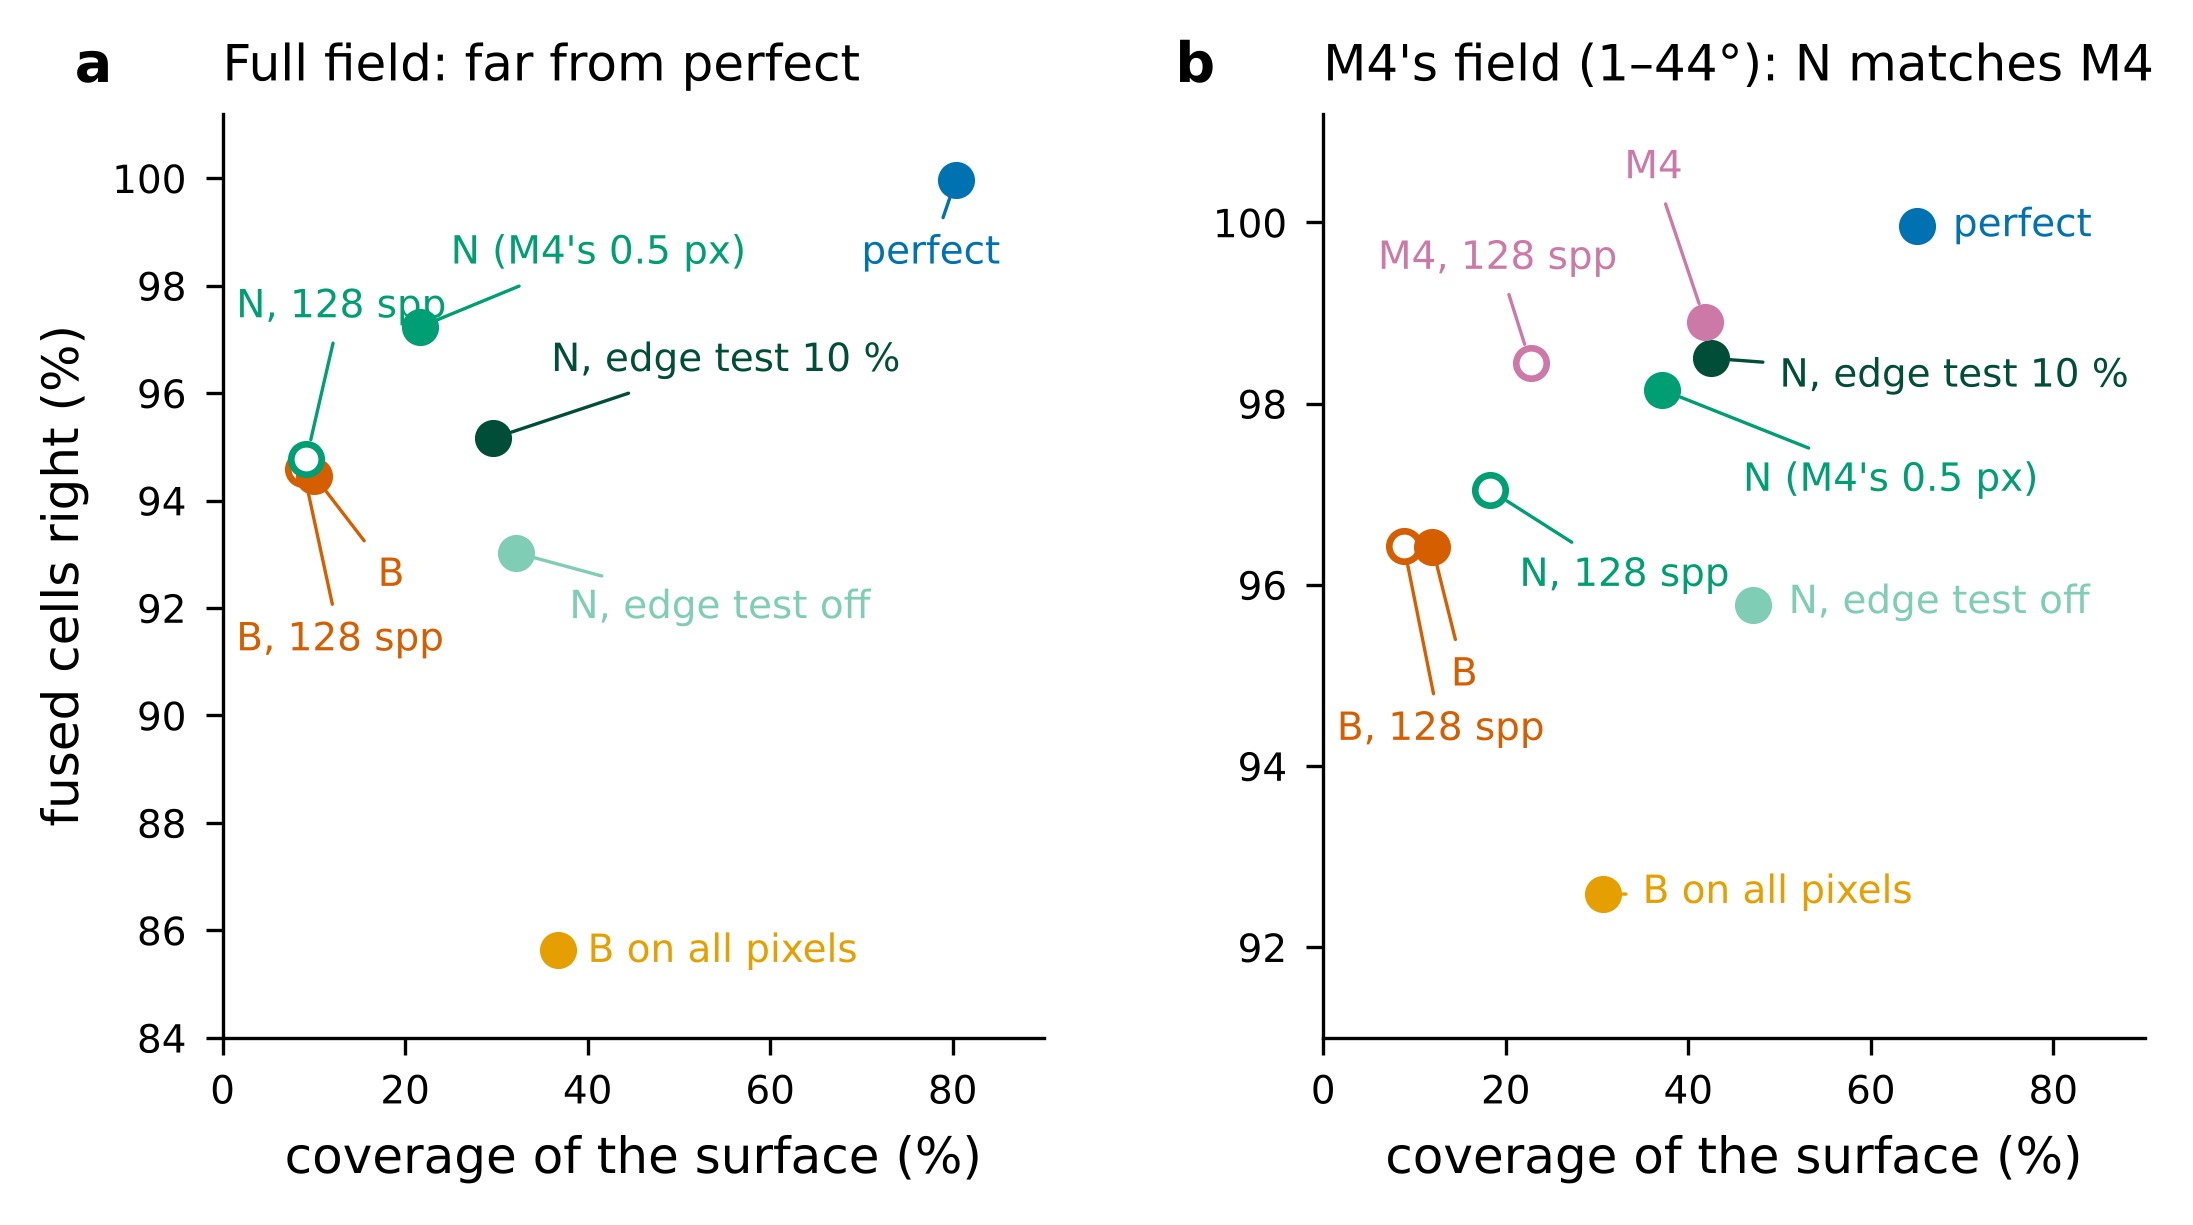
\includegraphics[width=\linewidth]{s11_precision.png}
\caption{Coverage against fused cells right, on the full field (a) and in M4's field (b). Open markers are 128-spp
renders. N's variants differ only in their depth-edge tolerance (Section~\ref{sec:diagnosis}). Code, workstation\WS;
drawn in the Chat sandbox.}\label{fig:precision}
\end{figure}

\begin{itemize}
\item \textbf{The coordinates are not the cause (C2).} In $18$--$44^\circ$ N covers 33.8\,\% at 99.25\,\% right, M4 35.5\,\%
  at 98.53\,\%. With the same matcher at the same noise, the panorama does what the foveated sensor does. Its control
  fails: B covers 11.7\,\% there.
\item \textbf{The sensor matters only near the heading.} In $1$--$18^\circ$ M4 covers 75.7\,\% against N's 50.4\,\%: the
  fovea's finer pixels, as expected. The perfect matcher covers 32.8\,\% there: with 0.5\,px of noise it is not a ceiling
  where pixels are fine.
\item \textbf{The matcher was the first cause (C3).} N covers 21.6\,\% of the full field against B's 10.1\,\%, more
  precisely (97.23 against 94.46\,\% right). Its control fails: N with the mirrored path's poses accepts 2,430 of
  2.35~million anchors, and none of its cells is right.
\item \textbf{Render noise was the second.} At 128 spp N is no better than B on the full field (9.2 against 8.8\,\%), and M4
  itself halves (41.9 to 22.7\,\% in its field) and fails its own classroom gate: 9.2\,\% coverage of its gate subset,
  against 36.8\,\% at 1024 spp. Noise matters for the NCC matchers and hardly for B (8.8 to 10.1\,\%), likely because
  B's cost averages over 101 looks.
\item \textbf{The yardstick was the third.} M4 was never compared with the perfect matcher. Even at 1024 spp it covers
  64\,\% of what the perfect matcher covers in its own field (41.9 of 65.0\,\%).
\item \textbf{Which pixels, and how they are scored.} On B's own anchors, N's cost covers less than B's but more precisely
  (8.3 against 10.1\,\%, at 97.59 against 94.46\,\% right): B's anchors, chosen by gradient, gather on depth edges, which N
  rejects (44\,\% of B's anchors on this path lay at true depth edges in stage 7c). Coverage grows with the pixels tried, for either cost: B's sweep on all of N's pixels covers 36.8\,\%, but at
  85.63\,\% right.
\end{itemize}

% ================================================================================================
\section{Where the gap lies}\label{sec:where}

Stage 11b scored every row by stage 9's sectors of the angle from the heading, by range, at depth edges or not, and by the
texture of each pixel. M4's texture measure (the rms gradient along the trace over the patch mean) counts noise as
texture, so the noise was removed. Cycles' noise falls as $1/\sqrt{\text{spp}}$, so the difference of the two renders of a
reference, the 128-spp one brought to the 1024-spp one's scale, has variance $9\sigma_{1024}^2$. The same operator
applied to both images gives the signal's share and the noise's. Against a noise-free render of a synthetic room, the
corrected measure is unbiased in median where noise dominates ($-0.7$\,\%, where the raw measure reads $+36$\,\%), and its
control (equal noise assumed in both renders) is off by $-100$\,\%\SB. The two renders' scalings differ by a gain of
0.973, which Code traced to their normalisation; their raw means agree to 0.1\,\%\WS.

\paragraph{Noise is a floor.} Even at 1024 spp, half of the surface's pixels have a gradient signal-to-noise ratio under
1.65, and about three in five of its cells lie under 3, though the texture is there (the signal's median is 0.081, four times M4's
threshold)\WS. With noise of the signal's size, even the true match's NCC falls below 0.8: below SNR 1, N covers 3.3\,\%
of the surface, the perfect matcher 84.8\,\% (Figure~\ref{fig:noise}a). Much of the perfect matcher's 80\,\% is coverage
that no image matcher could reach from these renders.

\paragraph{Beyond noise, the shortfall is to the side.} Against the perfect matcher kept only where SNR $\ge3$, a rough
ceiling, N reaches about 90\,\% in $15$--$60^\circ$ (30.3 against 34.1\,\%), 36\,\% in $60$--$120^\circ$ (15.9 against 44.2)
and 49\,\% in $120$--$165^\circ$ (17.0 against 34.4)\WS{} (Figure~\ref{fig:sectors}a). Where deep-motion's geometry is
strongest, M4's matcher is weakest.

\begin{figure}[t]
\centering
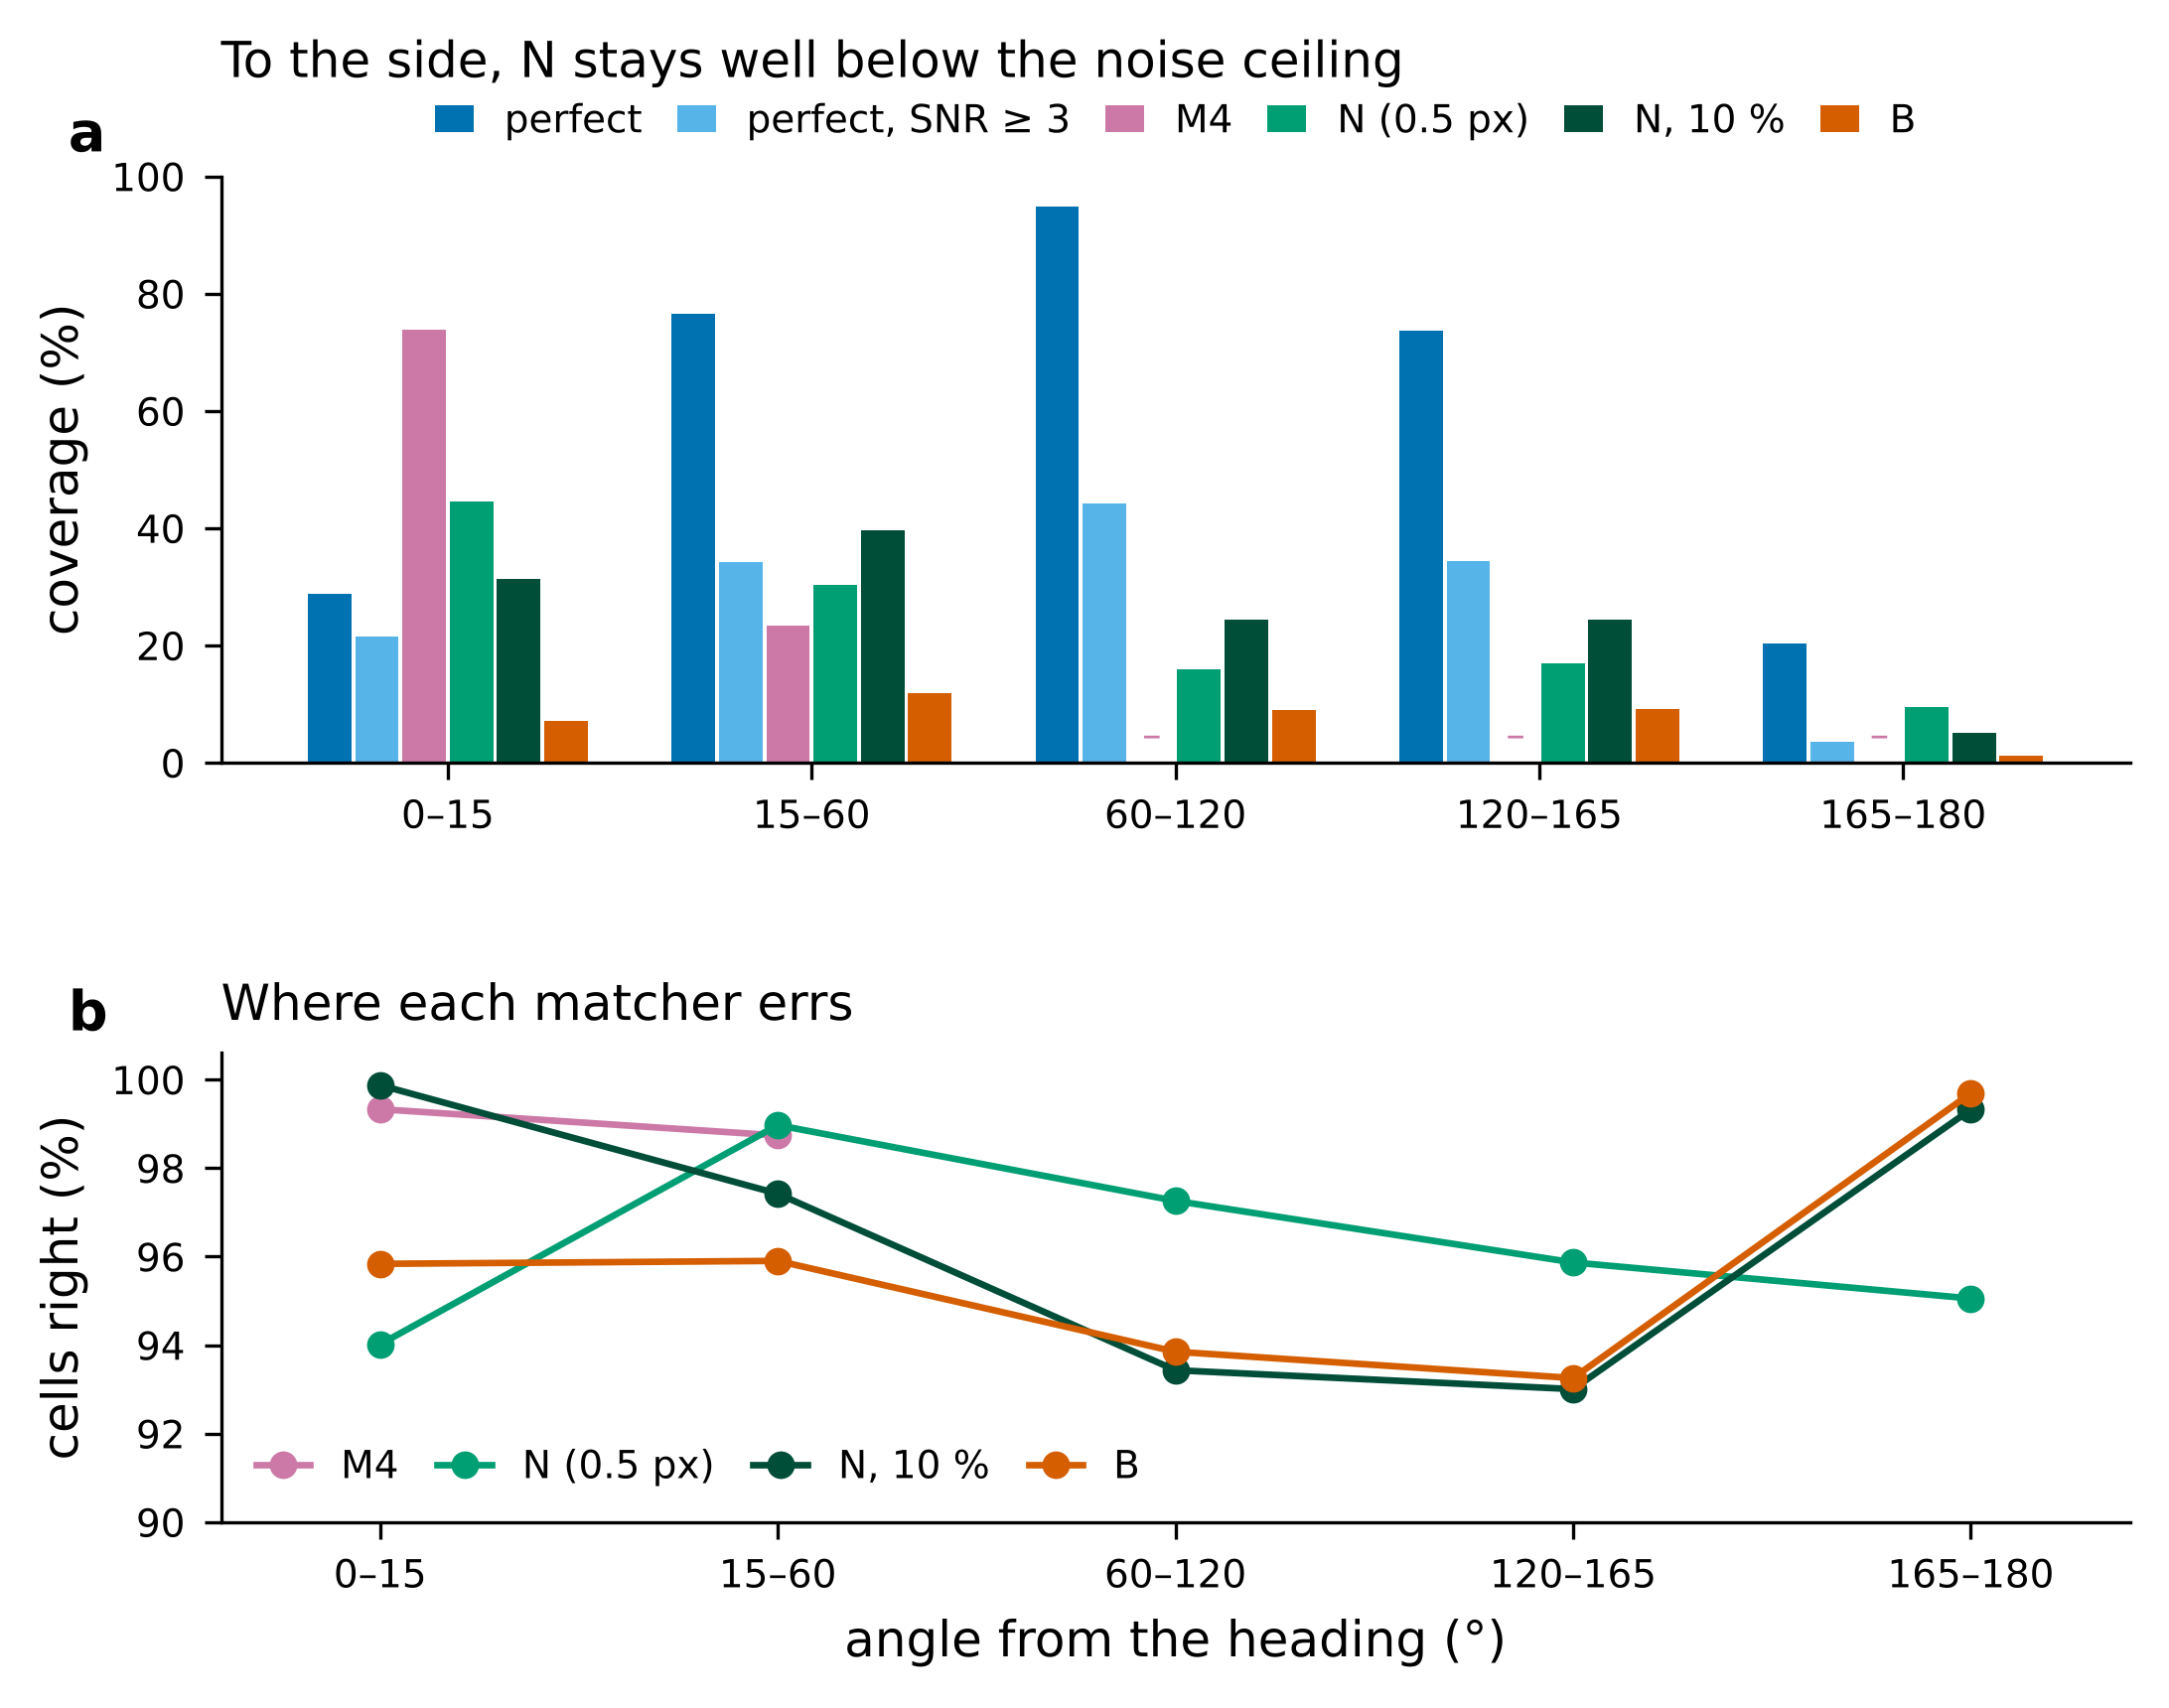
\includegraphics[width=\linewidth]{s11_sectors.png}
\caption{By angle from the heading: (a) coverage, with the perfect matcher kept where the gradient SNR is at least 3 as a
rough ceiling; (b) fused cells right. M4 sees only $1$--$44^\circ$: its $15$--$60^\circ$ bar holds its $15$--$44^\circ$
part. N's two depth-edge tolerances: M4's 0.5\,px and 10\,\% of $\zeta$ (Section~\ref{sec:diagnosis}). Code,
workstation\WS; drawn in the Chat sandbox.}\label{fig:sectors}
\end{figure}

\paragraph{One test does not carry over.} M4's depth-edge test rejects an anchor when a neighbour within $\pm3$\,px
deviates from its planar prediction by more than 0.5\,px of the longest step's displacement. Of its 433,295 rejections,
268,934 (62\,\%) fall on pixels that stage 9 calls interior\WS. The tolerance is in pixels, and the panorama's lateral
parallax is larger: about 57\,px per unit of inverse range to the side, against at most about 17 in M4's field. So
0.5\,px is about 1.6\,\% in inverse range at 1.8\,m to the side, and about 9\,\% in M4's field at 3\,m and $20^\circ$
(estimates from the two sensors' mappings): five times stricter in depth.

% ================================================================================================
\section{What the rest is}\label{sec:diagnosis}

Stage 11c re-ran N once, keeping every anchor's state before its last test, the depth edge, which feeds nothing back. That
one run gives three tolerances exactly: M4's 0.5\,px (which rebuilt the earlier N anchor for anchor, 301,581 accepted),
none, and 10\,\% of the inverse range, the ratio by which stage 9 calls a change of range an edge
(Table~\ref{tab:edge})\WS.

\begin{table}[h]
\centering\small
\begin{tabular}{@{}lccccc@{}}
\toprule
tolerance & full field & $1$--$44^\circ$ & $1$--$18^\circ$ & $18$--$44^\circ$ & rejected\\
\midrule
0.5\,px (M4's) & 21.6 (97.23) & 37.2 (98.15) & 50.4 (95.91) & 33.8 (99.25) & 433,295\\
10\,\% of $\zeta$ & 29.6 (95.16) & 42.4 (98.50) & 40.6 (99.92) & 41.7 (98.22) & 112,068\\
off & 32.1 (93.03) & 47.1 (95.77) & 54.5 (92.32) & 44.6 (97.07) & 0\\
\bottomrule
\end{tabular}
\caption{N with three depth-edge tolerances: coverage in \%, with cells right in brackets, and the anchors the test
rejects of the 734,876 that reach it. Code, workstation\WS.}\label{tab:edge}
\end{table}

\begin{itemize}
\item \textbf{The tolerance trades coverage for errors.} At 10\,\% N covers 29.6\,\% of the full field, nearly three times
  B, at 95.16\,\% right, two points less right than at 0.5\,px. In M4's field it is both more complete and more right than
  at 0.5\,px. Near the heading 10\,\% is the stricter tolerance, and 99.92\,\% right.
\item \textbf{Near and lateral surfaces fail beyond their SNR} (Figure~\ref{fig:noise}b,c). At equal SNR, from 1 up, N's
  NCC rejections fall with range (at SNR 3--10: 57, 41, 33 and 18\,\% from under 1\,m to over 3\,m) and peak to the side
  (at SNR 3--10: 44\,\% in $60$--$120^\circ$ against 13\,\% in $15$--$60^\circ$)\WS. That is the change of appearance over
  the window, largest for near points seen to the side: over $\pm0.5$\,m a point 1.8\,m away is seen across about
  $31^\circ$, and N's patch model (a shift, a slope along the trace, a gain and an offset) does not follow it. In the
  Classroom the near surfaces are also the lateral ones, so range and direction stay confounded.
\item \textbf{Clean lateral cells are wrong for every matcher.} In $60$--$120^\circ$ at SNR $\ge10$, N is 88.4\,\% right at
  0.5\,px and 76.5\,\% at 10\,\%, and B's sweep on all pixels 77.0\,\%\WS. High contrast gathers at true depth edges, so these
  are likely occlusion boundaries seen sideways, where one depth per anchor cannot be right on both sides. That is a
  reading, not a measurement.
\end{itemize}

\begin{figure}[t]
\centering
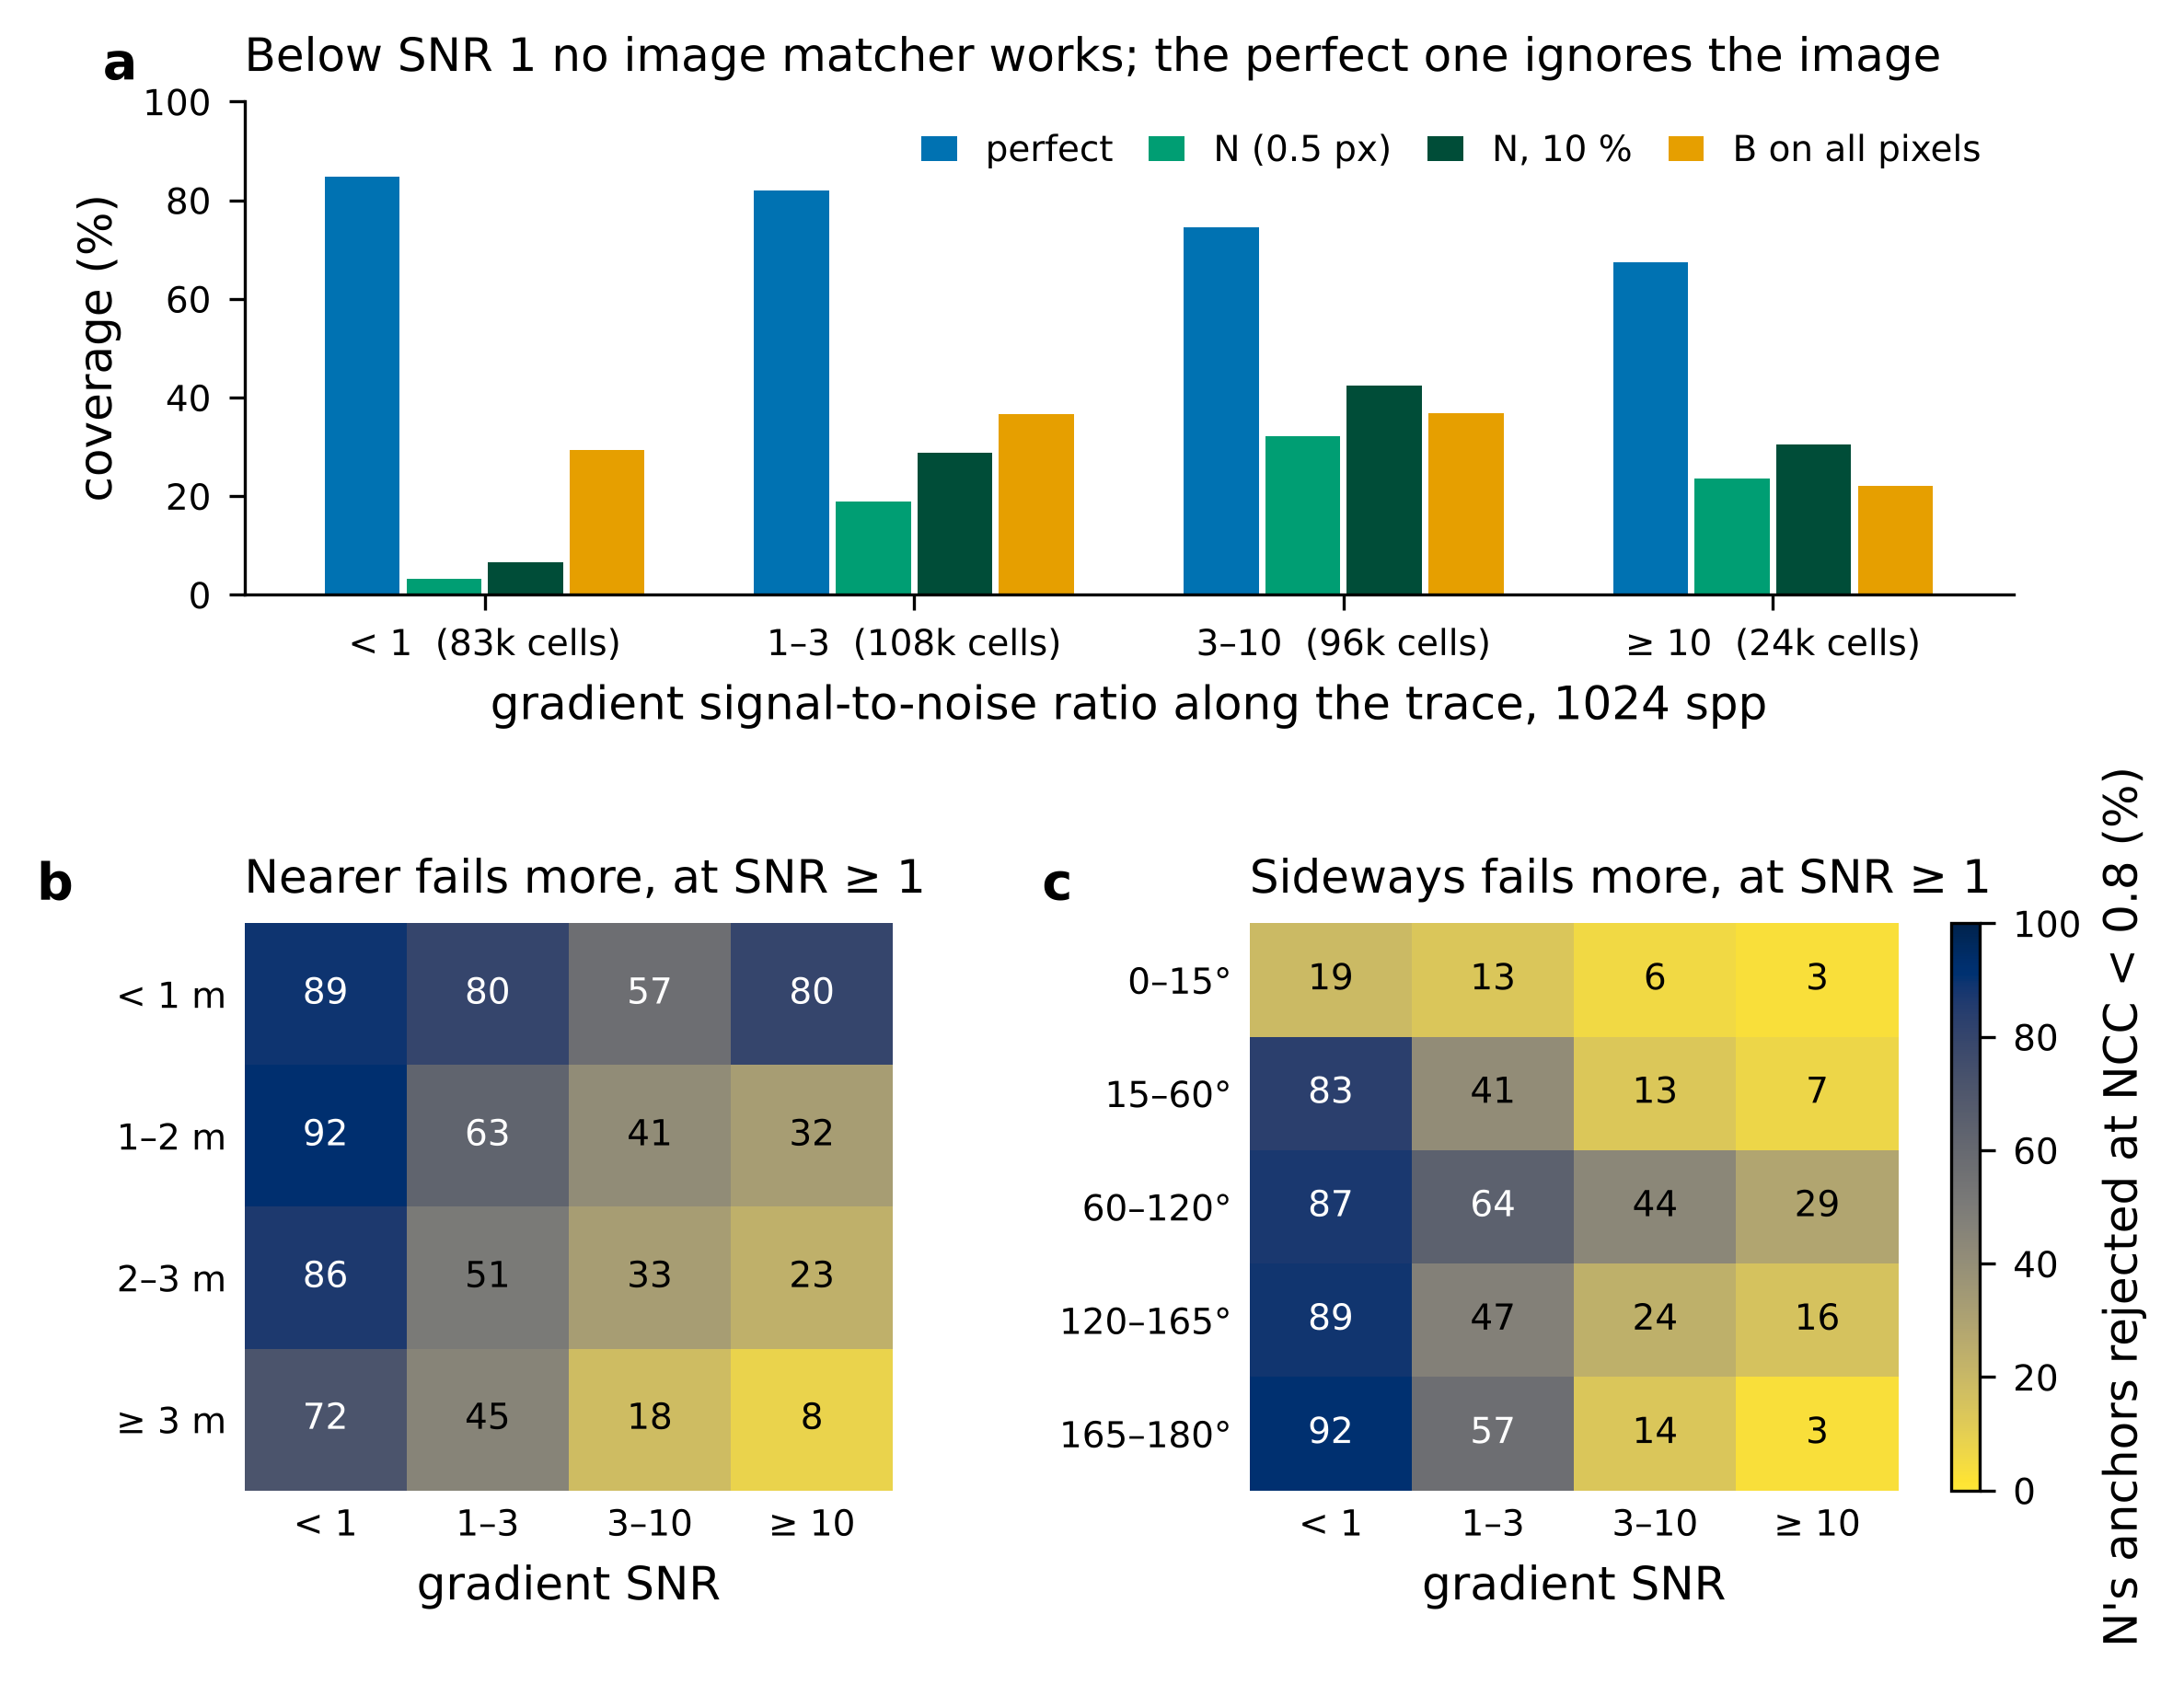
\includegraphics[width=\linewidth]{s11_noise.png}
\caption{(a) Coverage by the gradient's signal-to-noise ratio along the trace at 1024 spp; the perfect matcher ignores the
images. (b, c) The share of N's anchors rejected because their best mean NCC over the frames is under 0.8, by true range
and by angle from the heading, within each SNR class. Code, workstation\WS; drawn in the Chat sandbox.}\label{fig:noise}
\end{figure}

% ================================================================================================
\section{Conclusions}\label{sec:conclusions}

\begin{enumerate}
\item \textbf{The coordinates are not the cause.} With the same matcher and the same noise, the panorama does what the
  foveated sensor does outside the fovea. The \mt{} representation is cleared on the straight path.
\item \textbf{The sensor matters only near the heading,} where the fovea's finer pixels win.
\item \textbf{The comparison was unfair three times over:} a weaker matcher, renders with an eighth of the samples, and a yardstick
  that ignores the images.
\item \textbf{One rule had to be adapted:} M4's depth-edge tolerance in pixels, about five times stricter in depth on the
  panorama to the side.
\item \textbf{Two limits remain, and neither is the representation:} render noise, under which half of the surface cannot be
  matched from its images, and the change of appearance of near surfaces seen to the side over the window.
\end{enumerate}

% ================================================================================================
\section{Consequences}\label{sec:consequences}

\paragraph{Errors first.} The aim is a reconstruction without errors; coverage is secondary. The method builds the scene
incrementally, and the panorama sees the whole field at every look, so what one reference misses a later one can add. An
error, once in the model, stays. Judged so, none of the real matchers is good enough yet, but their errors are located:
\begin{itemize}
\item by direction: at 10\,\%, rays within $15^\circ$ of the heading or of its opposite are over 99\,\% right; rays to the
  side ($60$--$165^\circ$) about 93\,\%;
\item by contrast: the cleanest pixels are the least right (86\,\% at SNR $\ge10$), likely occlusion boundaries;
\item by range: at 10\,\%, 94.5\,\% right beyond 3\,m, 98\,\% under 2\,m;
\item by agreement: cells confirmed by two or more references are more right (N at 0.5\,px: 98.70 against 97.23\,\%; M4 in its
  field: 99.83\,\%).
\end{itemize}
So the natural rule for an incremental build is to accept a cell only once it is confirmed, and to let coverage come from
the full field and the length of the path, not from loose acceptance.

\paragraph{Choosing rays and depths.} Even with the panoramic sensor, the rays to process and the depths to consider can be
chosen. The rays that are reliable and those that carry the most parallax are not the same: the side has the most
information and the most errors. A sensing policy can trust the rays near the heading and its opposite, use side rays where
they are reliable (interior, moderate range, short windows) or only once confirmed, and bound each ray's depth search by
what is already built, which removes the far, ambiguous hypotheses. This is the information atlas of the M\"obius Traces note joined
to an action policy, now with measured error maps to drive it.

\paragraph{The matcher.} Three changes follow from the diagnosis: M4's matcher with acceptance tuned for errors, not
coverage; evidence from more frames against noise (the windows hold 101 looks and N uses 11; B used time without space, N
space with little time); and, for the side, patches warped fully by the hypothesis (slopes along and across the trace) with
windows suited to each ray's parallax, short for near lateral points.

\paragraph{A standard for the process.} The comparison went wrong because the two methods were run and judged under
different conditions. A standard fixes them per task: rendering (samples, resolution, noise model), path (primitives,
step), sensor (which rays, sampled how in space and time), matcher (windows, thresholds, depth envelope), fusion (the
confirmation rule), and evaluation (a gate on errors first, coverage second, reported by direction, range, depth edge and
noise level). It is the subject of the next document.

% ================================================================================================
\section{How the work was done}\label{sec:process}

As before, the N-Surface method~\cite{nsurface} in its light form: Claude in a chat sandbox (``Chat'') planned, wrote the
code and its checks and ran what a CPU can; Claude Code on the RTX~4090 workstation (``Code'') rendered and ran the
Classroom; Luiz asked the question, accepted the plan and its checks, and decided each next step. The checks were declared
before data, and two were amended before any data existed, when writing them out showed one control could not fail and
one test was two-sided where the question was one-sided. Each stage was dry-run first on a synthetic room of M4's fixture
planes, where both sensors could be ray-cast exactly. Code's reviews caught two of Chat's slips (a variant that was not
what had been defined, a breakdown that was missing) and checked an assumption instead of taking it (the gain between the
renders). The work in this note took one day, 21 November 2026.

\paragraph{Records.} Everything above is in \code{visgraf/deep-motion}~\cite{dm}, on the branch
\pth{experiment/p11-straight-cause}: \pth{docs/plan.md} (stage 11, its decision and its results), issue \#26, and the
records in \pth{docs/runs/dm-issue-26/}: \code{stage11.json}, \code{stage11b.json} and \code{stage11c.json}, the fixtures
and the logs. Figure sources are listed in \pth{figs/SOURCES.md}.

% ================================================================================================
\begin{thebibliography}{99}
\bibitem{dm} VISGRAF Lab. \emph{deep-motion}: depth from motion along curved paths.
  \url{https://github.com/visgraf/deep-motion}
\bibitem{mobius} Luiz Velho and Claude. ``M\"obius Traces: Depth from Motion along Curved Paths''. VISGRAF technical note,
  20 November 2026. \url{https://github.com/lvelho/foveal-depth-tr}
\bibitem{tr2} Luiz Velho and Claude. ``Foveated Vision on a Moving Head: Depth from Forward Motion''. VISGRAF technical
  note, 15 November 2026. \url{https://github.com/lvelho/foveal-depth-tr}
\bibitem{nsurface} Luiz Velho and Claude. ``The N-Surface Method: Rigor and Spontaneity in Human--AI Research''.
  VISGRAF technical note, 2026.
\end{thebibliography}

\end{document}
